\begin{frame}\label{sec:end}
\frametitle{Summary and Acknowledgments }%\hyperlink{slide_17}{\beamerbutton{back}}}

\begin{columns}[T]

\begin{column}[T]{0.3\textwidth}
\vspace{5pt}
\onslide<2->{\begin{figure}
    \centering
    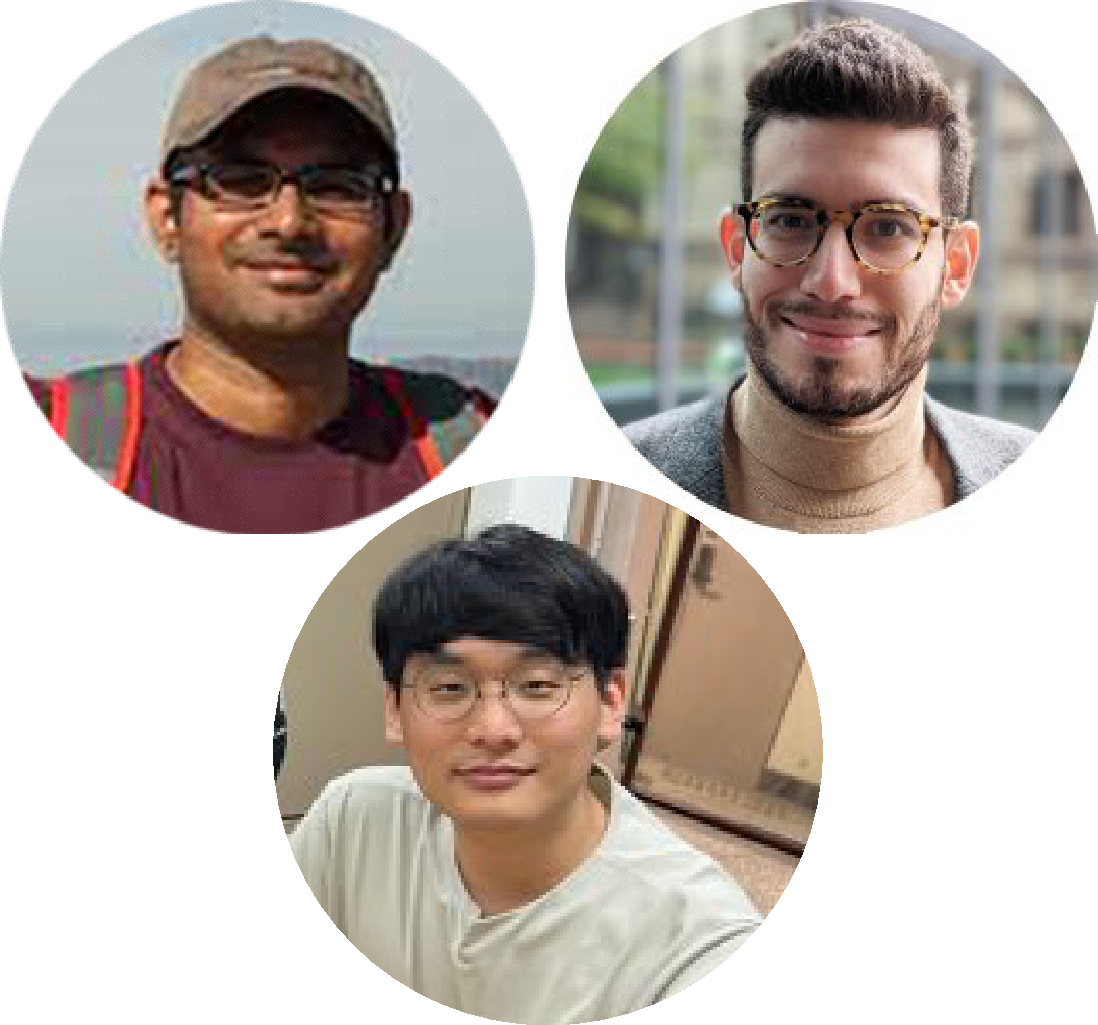
\includegraphics[width=0.825\linewidth]{acknowledgements/index.jpg}
    \caption{\centering \footnotesize{ \textbf{Advisor:} Kranthi K. Mandadapu  }}
    %\textbf{Co-workers:} Dimitrios Fraggedakis, Sanggeun Song}}
    %\\
    %\textbf{Paper:} \footnotesize } %
    \centering\includegraphics[width=0.8\linewidth]{acknowledgements/image912.png}
    \caption{\centering  \footnotesize{ \textbf{Funding:} DOE, Office of Basic Energy Sciences, Contract No. DEAC02-05CH11231}}
\end{figure}
}
\end{column}

\begin{column}[T]{0.7\textwidth}

\begin{figure}
    \centering\includegraphics[height=0.55\textheight]{a.2-intro_dftheory/DF_Theory_Excitations_Zoom_2.pdf}
    \hspace{1em}
    \centering\includegraphics[height=0.55\textheight]{d.6-fac_results_3/persistlowT3.png}
    
    \caption{A self-consistent model of glassy dynamics based on excitations and elasticity $\to$ excitation-driven glassy dynamics. Future work: \textbf{3D} %, \textbf{Radius of Gyration}.
    \onslide<3->{\textbf{Paper:} M.R. Hasyim, K.K. Mandadapu,  \textit{J. Chem. Phys.} 155, 044504 (2021); M.R. Hasyim, K.K. Mandadapu, \texttt{arXiv:2310.06584} (2023)}
    }
\end{figure}
\vspace{-1.0em}
% D. Fraggedakis, M,R. Hasyim, K.K. Mandadapu.  120.14 \textit{Proc. Natl. Acad. Sci. U.S.A.} (2023); 
%\vspace{20em}
\onslide<4->{\vspace{-0.5em}\Huge \textbf{Questions?}}%e-mail at \texttt{muhammad\_hasyim@berkeley.edu}}
\end{column}

\end{columns}
\end{frame}